We perform experiments to show that MoIE-CXR 1) captures a diverse set of concepts, 2) does not compromise BB's performance, 3) covers ``harder'' instances with the residuals in later iterations resulting in their drop in performance, 4) is finetuned well to an unseen domain with minimal computation. 

\begin{figure*}[ht]
\begin{center}
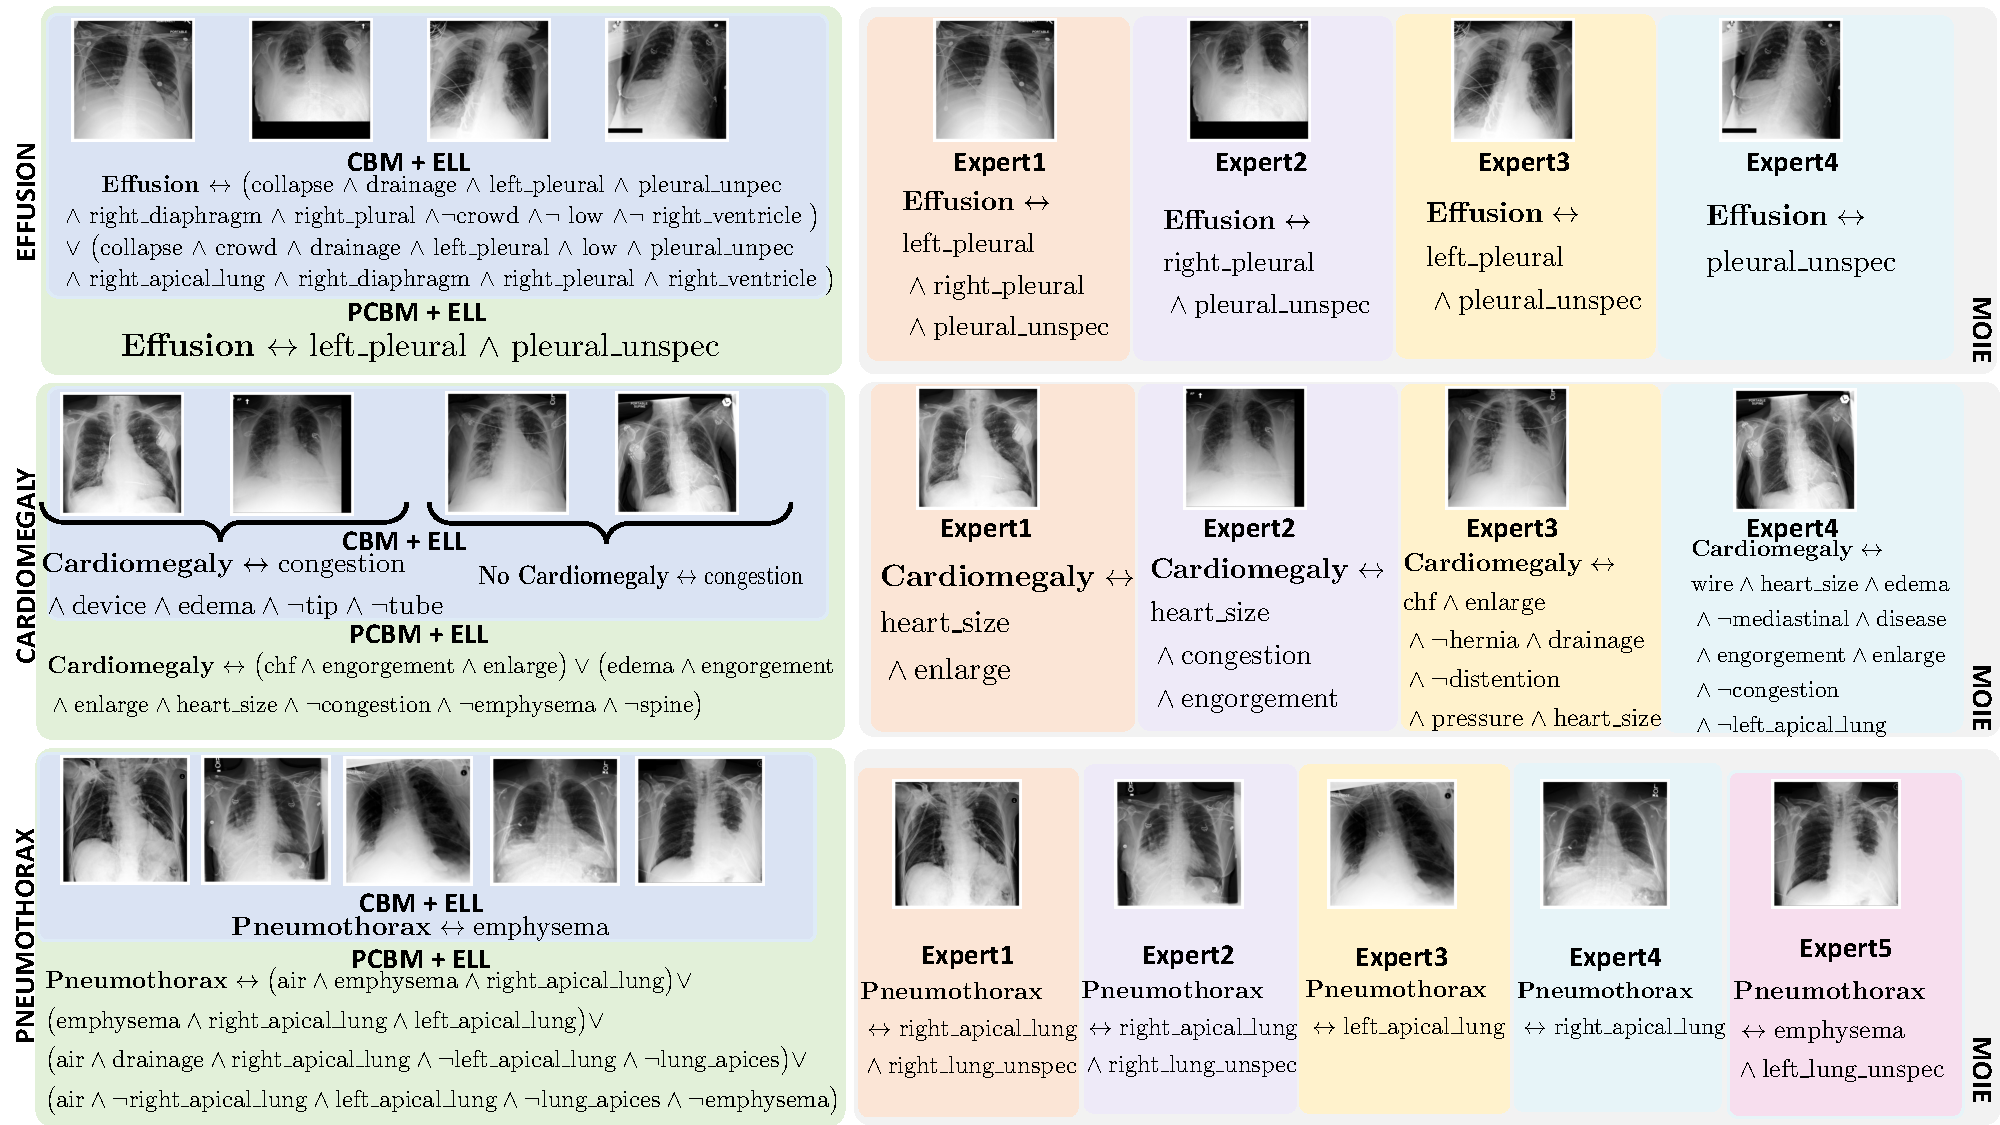
\includegraphics[width=\linewidth]{plots/main/Qual_main_up.pdf}
\caption{Qualitative comparison of MoIE-CXR discovered concepts with the baselines.}
\label{fig:qual}
\end{center}
\end{figure*}

\noindent \textbf{Experimental Details.} We evaluate our method using  220,763 frontal images from the MIMIC-CXR dataset \cite{12_johnsonmimic}. We use Densenet121 \cite{huang2017densely} as BB ($f^0$) to classify cardiomegaly, effusion, edema, pneumonia, and pneumothorax, considering each to be a separate binary classification problem. We obtain 107 anatomical and observation concepts from the RadGraph’s inference dataset~\cite{10_jain2021radgraph}, automatically generated by DYGIE++~\cite{23_wadden-etal-2019-entity}. We train BB following~\cite{yu2022anatomy}. To retrieve the concepts, we utilize until the $4^{th}$ Densenet block as feature extractor $\Phi$ and flatten the features to learn $t$. We use an 80\%-10\%-10\% train-validation-test split with no patient shared across splits. We use 4, 4, 5, 5, and 5 experts for cardiomegaly, pneumonia, effusion, pneumothorax, and edema. We employ ELL~\cite{barbiero2022entropy} as $g$. Further, we only include concepts as
input to $g$ if their validation auroc exceeds 0.7. Refer to Tab. 1 in the supplementary material for the hyperparameters. 
% We train the model on a single NVIDIA GPU-32G of memory. 
We stop until all the experts cover at least 90\% of the data cumulatively. \noindent \textbf{Baseline.} We compare our method with 1) end-to-end CEM~\cite{zarlenga2022concept}, 2) sequential CBM~\cite{koh2020concept}, and 3) PCBM~\cite{yuksekgonul2022post} baselines, comprising of two parts: a) concept predictor $\Phi: \mathcal{X} \rightarrow \mathcal{C}$, predicting concepts from images, with all the convolution blocks; and b) label predictor, $g: \mathcal{C} \rightarrow \mathcal{Y}$, predicting labels from the concepts. We create CBM + ELL and PCBM + ELL by replacing the standard classifier with the identical $g$ of MOIE-CXR to generate FOLs~\cite{barbiero2022entropy} for the baseline.